\chapter{Teorie - Astronomické měření}
\label{3-teorie-astronomickeho-mereni}
Astronomické měření bylo na našem území prováděno od roku 1863 do roku 1974. Metody měření se v~průběhu času měnily v~závislosti na aktuálním vědeckém poznání a na přesnosti, s~jakou bylo možno určovat čas. Například měření zeměpisné délky vztažené k~základnímu poledníku byla započata až roku 1927, díky existenci rádiových časových signálů. Astronomické měření bylo prováděno především v~rámci astronomicko-geodetické sítě (AGS). Body, u~nichž byly určeny astronomické země\-pisné souřadnice a astronomický azimut, se nazývají Laplaceovy body \cite{kostelecky_geodeticka_astronomie}.

\section{Astronomické azimuty}
V~rámci výuky Teoretické geodézie na FSv ČVUT se měří pouze astronomické \text{azimuty} Slunce metodou určení hodinového úhlu, a tak zde bude zmíněn pouze požadavek přesnosti určení času pro toto měření. Výpočet astronomického azimutu vychází se vztahu:

\begin{equation}    
\tg{(A)} = \frac{\sin(t)}{\sin(\varphi) \cdot \cos(t) - \cos(\varphi) \cdot \tg(\delta)}
\end{equation}

kde \(\delta\) je deklinace Slunce a lze ji zjistit například z~astronomických tabulek\\
a \(t\) je hodinový úhel získaný ze vztahu:

\begin{equation}
    t = S+\lambda-\alpha
\end{equation}

kde \(\alpha\) je rektascenze Slunce a lze ji zjistit například z~astronomických tabulek\\

\(S\) je pravý světový hvězdný čas, který je ovlivněn precesí i nutací a lze jej \text{dopočítat} z~různých časů pomocí vztahů popsaných v~kapitole 3 \cite{kostelecky_geodeticka_astronomie}. Způsob převodu mezi různými časy je naznačen zde: 

\begin{figure}[H]
    \centering
    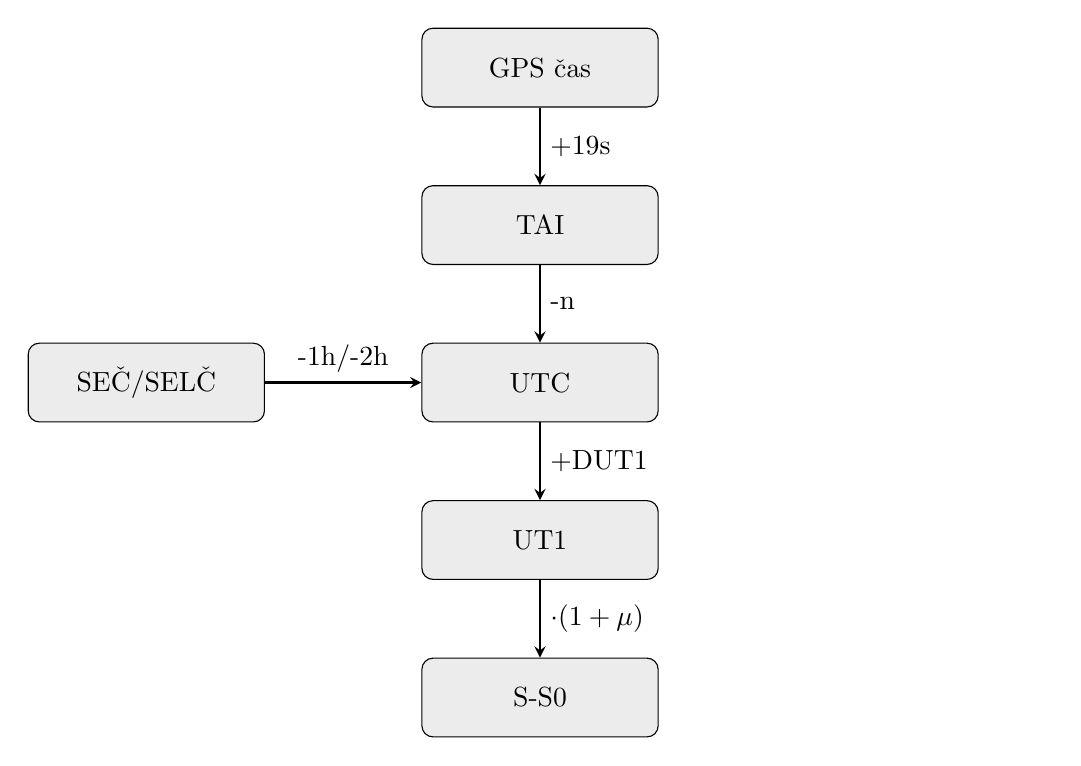
\begin{tikzpicture}[node distance=2cm]
        \tikzstyle{startstop} = [rectangle, rounded corners, minimum width=3cm, minimum height=1cm,text centered, draw=black, fill=lightgray!30]
        \tikzstyle{arrow} = [thick,->,>=stealth]
        
        \node (GPST) [startstop] {GPS čas};
        \node (TAI) [startstop, below of=GPST] {TAI};
        \node (UTC) [startstop, below of=TAI] {UTC};
        \node (SECS) [startstop, left of=UTC, xshift=-3cm, anchor=center] {SEČ/SELČ};
        \node (nev) [startstop, right of=UTC, xshift=3cm, anchor=center, fill=white, draw=white] {}; % Neviditelný uzel bílý obrys
        \node (UT1) [startstop, below of=UTC] {UT1};
        \node (S_S0) [startstop, below of=UT1] {S-S0};
        
        \draw [arrow] (GPST) -- node[right] {+19s} (TAI);
        \draw [arrow] (TAI) -- node[right] {-n} (UTC);
        \draw [arrow] (SECS) -- node[above] {-1h/-2h} (UTC);
        %\draw [arrow] (nev) -- (UTC); % Šipka z neviditelného uzlu na UTC
        \draw [arrow] (UTC) -- node[right] {+DUT1} (UT1);
        \draw [arrow] (UT1) -- node[right] {\(\cdot (1+\mu)\)} (S_S0);
    \end{tikzpicture}
    \small
    \\
    *\(S_0\) je světový hvězdný čas pro 0h UT1 [h] v~den pozorováni\\
    *\(\mu\) lze dohledat v~astronomických tabulkách
    \caption{Schéma konverze časových údajů}
\end{figure}


Do výpočtu tedy vstupují zeměpisné souřadnice stanoviska a čas měření na Slunce, zbylé hodnoty lze zjistit z~astronomických tabulek a bulletinu mezinárodní služby IERS. Experimentálním dosazením hodnot do vztahů (4.1) pro zeměpisné souřadnice stanoviska 50° s. š. a 15° v. d. a hodnot vycházejících z~časů UTC lišících se o~1s 0.1s a 0.01s byl orientačně zjištěn vliv chyby v~určení času na výsledný astronomický azimut Slunce.


\begin{table}[H]
    \centering
    \caption{Rozdíly azimutů Slunce v~závislosti na rozdílu časů UTC}
    \begin{tabular}{|c|c|c|}
    \hline
    \( \Delta \) UTC [s] & Rozdíl azimutů ["] & Rozdíl azimutů [\(^{cc}\)] \\
    \hline \hline
    1    & 13.93 & 43.01 \\ \hline
    0.1  &  1.39 & 4.30  \\ \hline
    0.01 &  0.13 & 0.43  \\ \hline
    \end{tabular}
\end{table}

Z~tabulky vyplývá, že aby byla chyba v~určení azimutu Slunce menší než jedna úhlová vteřina, je potřeba určovat čas s~přesností na setiny sekund.